\documentclass[12pt,titlepage]{article}
\usepackage[margin=1.25in]{geometry}
\usepackage{graphicx,amsmath,blindtext,longtable,tabu,enumitem,wrapfig}

%% Variables definition
\newcommand{\vSubject}{Critical Thinking and Problem Solving}
\newcommand{\vSubtitle}{Task and Assignment}
\newcommand{\vName}{Dicha Zelianivan Arkana}
\newcommand{\vNIM}{2241720002}
\newcommand{\vClass}{1i}
\newcommand{\vDepartment}{Information Technology}
\newcommand{\vStudyProgram}{D4 Informatics Engineering}

%% [START] Tikz related stuff
\usepackage{tikz}
\usetikzlibrary{svg.path,calc,shapes.geometric}
\tikzstyle{terminator} = [rectangle, draw, text centered, rounded corners = 1em, minimum height=2em]
\tikzstyle{process} = [rectangle, draw, text centered, minimum height=2em]
\tikzstyle{decision} = [diamond, draw, text centered, minimum height=2em]
\tikzstyle{data}=[trapezium, draw, text centered, trapezium left angle=60, trapezium right angle=120, minimum height=2em]
\tikzstyle{connector} = [line width=0.5mm,->]
%% [END] Tikz related stuff

%% [START] Fancy header related stuff
\usepackage{fancyhdr}
\pagestyle{fancy}
\setlength{\headheight}{15pt} % compensate fancyhdr style
\fancyhead{}
\fancyfoot{}
\fancyfoot[L]{\thepage}
\fancyfoot[R]{\textit{\vSubject - \vSubtitle}}
\renewcommand{\footrulewidth}{0.4pt}% default is 0pt, overline for footer
%% [END] Fancy header related stuff

%% [START] Custom tabular command related stuff
\usepackage{tabularx}
\newcommand{\details}[2]{
    #1 & #2  \\
}
%% [END] Custom tabular command related stuff

%% [START] Figure related stuff
\newcommand{\image}[3][1]{
    \begin{figure}[h]
        \centering
        \includegraphics[#1]{#2}
        \caption{#3}
        \label{#3}
    \end{figure}
}
%% [END] Figure related stuff

\begin{document}
\begin{titlepage}
    \centering
    \vfill
    {\bfseries\LARGE
        \vSubject\\
        \vskip0.25cm
        \vSubtitle
    }
    \vfill
    
\includegraphics[width=6cm]{images/polinema-logo.png}
    \vfill
    {
        \textbf{Name}\\
        \vName\\
        \vskip0.5cm
        \textbf{NIM}\\
        \vNIM\\
        \vskip0.5cm
        \textbf{Class}\\
        \vClass\\
        \vskip0.5cm
        \textbf{Department}\\
        \vDepartment\\
        \vskip0.5cm
        \textbf{Study Program}\\
        \vStudyProgram
    }
\end{titlepage}

\section{Task - Page 33}
\begin{enumerate}
    \item {
        Consider something you might want to buy, such as a car, cell phone, or computer. 
        List the information you need to make a decision about the model or certain type to buy.

        I want to buy a new laptop to replace my old one, so it needs to be better. The informations that I need to pay attention are:
        \begin{itemize}
            \item The processor type, whether it's AMD Ryzen or Intel
            \item The screen type, whether it's an IPS or TN, it needs to be at least IPS
            \item The screen resolution, it needs to have at least FHD (1920x1080) resolution
            \item The amount of storage, it needs to be at least 256GB M.2 NVME SSD
            \item The amount of RAM, it needs to be at least 8GB 3200Mhz
            \item The brand, it needs to be a well-known brand
        \end{itemize}
    }
    \item {
        The gasoline use of a number of cars has been measured. 
        Each car starts with a full tank, then travels (all travels on the same road). 
        After the trip the tank is refilled, the amount of gasoline needed to fill it is recorded.
        The results are shown below. Sort the car's fuel efficiency (km/liter), from lowest to highest.

        \begin{table}[h]
            \caption{Unsorted Data}
            \begin{longtabu} to \textwidth {|l|c|c|}
                \hline \multicolumn{1}{|c|}{\textbf{Car}} & \multicolumn{1}{c|}{\textbf{Length of Journey (km)}} & \multicolumn{1}{c|}{\textbf{Petrol Used (Litres)}} \\ \hline 
                \endfirsthead

                Montevideo & 120 & 10 \\
                Stella & 150 & 16 \\
                Riviera & 200 & 25 \\
                Roamer & 185 & 21 \\
                Carousel & 230 & 16 \\
                
                \hline
            \end{longtabu}

            \setcounter{table}{1}

            \caption{Sorted Data}
            \begin{longtabu} to \textwidth {|l|c|c|c|}
                \hline \multicolumn{1}{|c|}{\textbf{Car}} & \multicolumn{1}{c|}{\textbf{Length of Journey (km)}} & \multicolumn{1}{c|}{\textbf{Petrol Used (Litres)}} & \multicolumn{1}{c|}{\textbf{Efficiency (km/litre)}} \\ \hline 
                \endfirsthead

                Carousel & 230 & 16 & $230/16=14.375l$ \\
                Montevideo & 120 & 10 & $120/10=12l$ \\
                Stella & 150 & 16 & $150/16=9.375l$\\
                Roamer & 185 & 21 & $185/21=8.8l$\\
                Riviera & 200 & 25 & $200/25=8l$ \\

                \hline
            \end{longtabu}
        \end{table}
    }
    \pagebreak
    \item {
        The pie chart below illustrates the changing introduction of CDs in 1985 in
        the recorded music market. The total annual sales of all types of records in
        1984 was 170 million and in 1994 they were 234 million. What do you think
        happened to the actual annual sales of vinyl singles between 1984 and
        1994?

        \begin{figure}[h]
            \centering
            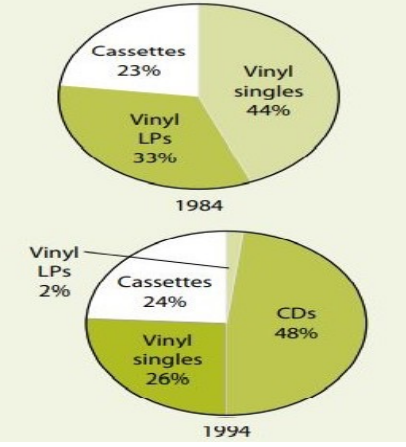
\includegraphics[width=0.5\textwidth]{./images/cd-pie-chart.png}
            \caption{Pie Chart}
        \end{figure}

        From this chart, we can gather up some data. Since on the pie chart it is represented using percentage, we can multiply it with the actual number.
        After done calculating them, we can visualise the data using a table as such:

        \setcounter{table}{2}
        \begin{table}[h]
            \caption{Annual Sales of All Types of Records}
            \begin{longtabu} to \textwidth {|l|r|r|}
                \hline \multicolumn{1}{|c|}{\textbf{Type}} & \multicolumn{1}{c|}{\textbf{1984}} & \multicolumn{1}{c|}{\textbf{1994}} \\ \hline 
                \endfirsthead

                Cassettes & $23\%\times170M=39.1M$ & $24\%\times234M=56.16M$ \\
                Vinyl Singles & $44\%\times170M=74.8M$ & $26\%\times234M=60.8M$ \\
                Vinyl LPs & $33\%\times170M=56.1M$ & $2\%\times234M=4.68M$ \\
                CD & - & $48\%\times234M=112.32M$ \\

                \hline
            \end{longtabu}
        \end{table}

        From this table, we can make a conclusion that the annual sales of vinyl singles between 1984 and 1994 went down 14 million
    }
    \pagebreak
    \item {
        Pancake stall selling sweet pancakes and savory pancakes. Savory pancakes
        can have three toppings (eggs, ham, tomatoes) that can be used in any
        combination. The sweet ones are topped with marmalade (orange jam),
        lemon or strawberry with ice cream or fresh cream. How many combinations
        does the kiosk sell?

        From the text above, we can gather up these data:
        \begin{itemize}
            \item Sweet and Savory pancakes
            \item Savory pancake toppings (eggs, ham, tomatoes), can be used in any combinations
            \item Sweet pancake topppings (marmalade, lemon or strawberry with ice cream or fresh cream)
        \end{itemize}

        The final result would be:
        \begin{itemize}
            \item {
                There are 7 savory pancake combinations
                \begin{itemize}
                    \item eggs
                    \item ham
                    \item tomatoes
                    \item eggs, ham
                    \item eggs, tomatoes
                    \item ham, tomatoes
                    \item eggs, ham, tomatoes
                \end{itemize}
            }
            \item {
                There are 5 sweet pancake combinations
                \begin{itemize}
                    \item marmalade
                    \item lemon with ice cream
                    \item lemon with fresh cream
                    \item strawberry with ice cream
                    \item strawberry with fresh cream
                \end{itemize}
            }
        \end{itemize}

        All in all, there are 12 combinations for sweet and savory pancake.
    }
\end{enumerate}

\section{Assignment - Page 64}
\begin{enumerate}
    \item {
        If the distance from Jakarta to Ontario – Canada is exactly 14000 km, a plane takes 22 hours to depart.
        Meanwhile, from Ontario to Jakarta, the time needed is only 17 hours due to the wind conditions blowing in the
        direction of the plane's speed. Assuming the aircraft is moving at a constant speed in both directions of flight
        (depart \& return) and in stable clear air without clouds, what is the average wind speed on that flight?

        From the text above, these are the informations that we can gather:
        \begin{itemize}
            \item Distance from Jakarta to Ontario is exactly 14000km
            \item {
                It takes 22 hours for a plane to depart from Jakarta to Ontario.\\
                Which means it flies opposite to the wind direction, we need to reduce its speed with the wind speed.
            }
            \item {
                It takes 17 hours for a plane to depart from Ontario to Jakarta.\\
                Which means it flies opposite to the wind direction, we need to reduce its speed with the wind speed.
            }
        \end{itemize}

        Let $x=plane~speed$ and $y=wind~speed$. We can calculate as such:
        \begin{align*}
            17(x+y) &= 14000 \\
            22(x-y) &= 14000 \\~\\
            17x + 17y &= 14000 \\
            22x - 22y &= 14000 \\~\\
            374x + 374y &= 308000 \\
            374x - 374y &= 238000 \\~\\
            748x &= 546000 \\~\\
            x &= \frac{546000}{748} = 730~(rounded) \\~\\
        \end{align*}
        \begin{align*}
            17(x+y) &= 14000 \\~\\
            17x + 17y &= 14000 \\~\\
            17(730) + 17y &= 14000 \\~\\
            12410 + 17y &= 14000 \\~\\
            17y &= 14000 - 12410 \\~\\
            17y &= 1590 \\~\\
              y &= \frac{1590}{17} = 93.5~(rounded) \\~\\
        \end{align*}
        From the calculation above, we can conclude that the wind speed is 93.5 km/h
    }
    \pagebreak
    \item {
        Yasmin has been saving for a long time to buy a gift for her sister's birthday. Every time he has coins with a
        face value of 5 cents and 20 cents, he puts them into his piggy bank. Today he broke his piggy bank and counted
        all the money in it. He calculated by stacking the coins so that they became piles worth 1 USD in each pile.
        When he finished, he realized that the piles of coins he made were of different heights. If 1 USD = 100
        cents, and if the 5 cent vs 20 cent coin thickness is exactly the same, then how many stack classes are there
        based on their height?

        These are the informations that we can gather from the text above:
        \begin{itemize}
            \item Everytime he has coins with a face value of 5 cents and 20 cents, he puts them into his piggy bank
            \item Each pile worth 1 USD
            \item The piles were of different heights
            \item 1 USD = 100 cents
            \item The thickness of the coin is exactly the same.
        \end{itemize}

        We can visualise the possible combinations using a table, assuming their height is 1mm:
        \setcounter{table}{3}
        \begin{table}[h]
            \caption{Table of Possible Combinations}
            \begin{longtabu} to \textwidth {|c|c|c|c|}
                \hline \multicolumn{1}{|c|}{\textbf{No.}} & \multicolumn{1}{c|}{\textbf{5 cents}} & \multicolumn{1}{c|}{\textbf{20 cents}} & \multicolumn{1}{c|}{\textbf{Height}} \\ \hline 
                \endfirsthead

                1 & $20\times$ & - & $20mm$ \\
                2 & $16\times$ & $1\times$ & $17mm$ \\
                3 & $12\times$ & $2\times$ & $14mm$ \\
                4 & $8\times$ & $3\times$ & $11mm$ \\
                5 & $4\times$ & $4\times$ & $8mm$ \\
                6 & - & $5\times$ & $5mm$ \\

                \hline
            \end{longtabu}
        \end{table}

        From this table, we can make a conclusion that there are 6 stack classes based on their height.
    }
    \pagebreak
    \item {
        At the bank where I deposit money, the ATM pin consists of a 4-digit number. It can be very difficult to always
        remember the Pin. To make it easier to remember, I created my ATM pin in the following way:
        \begin{itemize}
            \item The first 2 digits are my date (day) of birth, reversed.
            \item The remaining 2 digits are my birth month, reversed as well.
            \item If the date or month is 1 digit, then 0 is added before it is reversed.
        \end{itemize}
        Which of the following PINs CANNOT be my PIN?
        \begin{enumerate}[label=\Alph*.]
            \item 3221
            \item 5060
            \item 1141
            \item 2121
            \item 1290
        \end{enumerate}
        
        We can decode those PINS back to its original form using the rules above and verify if the date or the month is valid.
        \begin{enumerate}[label=\Alph*.]
            \item 3221 $\rightarrow$ The date is 23 and the month is 12 $\rightarrow$ Valid
            \item 5060 $\rightarrow$ The date is 5 and the month is 6 $\rightarrow$ Valid
            \item 1141 $\rightarrow$ The date is 11 and the month is 14 $\rightarrow$ Invalid
            \item 2121 $\rightarrow$ The date is 12 and the month is 12 $\rightarrow$ Valid
            \item 1290 $\rightarrow$ The date is 21 and the month is 9 $\rightarrow$ Valid
        \end{enumerate}
        
        The \textbf{C} option is invalid, because on our calendar system, the month can only go up to 12 which is December. 
        There is no 14th month.
    }
    \item {
        I went to buy fruit at a market in Waylandpuro and asked one of the fruit sellers there: “Sir, how much do you buy 1
        orange for?”. The seller said, 1 orange plus 1 lemon costs Rp.2000. Then he said again (which confused me even more), if
        1 lemon equals 1 grapefruit it becomes Rp.3000. He said the price of each fruit is different. Based on this unhelpful
        information, which of the following can be confirmed?
        \begin{enumerate}[label=\Alph*.]
            \item 1 orange is more expensive than 1 lemon
            \item 1 lemon is more expensive than 1 grapefruit
            \item 1 grapefruit costs more than Rp.1000
            \item 1 orange costs less than Rp.1000
        \end{enumerate}
        \pagebreak
        From the unhelpful information above, we can gather up these data:
        \begin{itemize}
            \item 1 orange + 1 lemon = 2000
            \item If 1 lemon = 1 grapefruit, then it becomes 3000
            \item Each fruit price is different
        \end{itemize}

        From the information above, we can say that \textbf{1 grapefruit costs more than Rp.1000} because there's a statement which says
        \textit{if 1 lemon equals 1 grapefruit it becomes Rp.3000}, which means each grapefruit could cost Rp.3000 which is more than Rp.1000
    }
\end{enumerate}

\section{Task - Page 85}
\begin{enumerate}
    \item {
        The solid on the right (figure \ref{prism}), a cube with two corners cut off, is made of a piece of cardboard
        that is shaped and folded. (The dotted line represents the hidden edge.)
        Which of the following folds of cardboard (figure \ref{prismpaper}) is suitable for creating the shape?

        \begin{figure}[h]
            \centering
            \begin{minipage}{.4\textwidth}
                \centering
                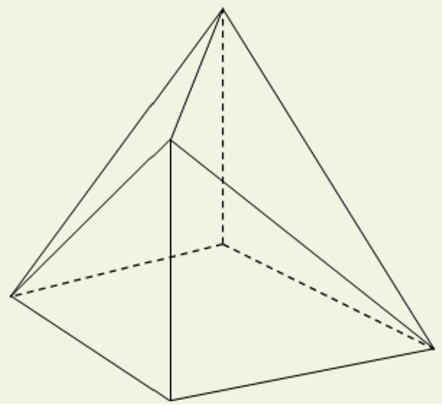
\includegraphics[width=\textwidth]{./images/prism.png}
                \caption{Cube with two corners cut off}
                \label{prism}
            \end{minipage}
            \hspace{0.5cm}
            \begin{minipage}{.4\textwidth}
                \centering
                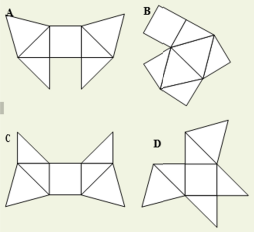
\includegraphics[width=\textwidth]{./images/prism-papers.png}
                \caption{Cardboards}
                \label{prismpaper}
            \end{minipage}
        \end{figure}

        To determine which cardboard fold is suitable, we can imagine how each cardboard folds will form.
        \begin{enumerate}[label=\Alph*.]
            \item Unsuitable, because the left and right part will overlap with each other
            \item Suitable, there will be no overlap and it will form a cube with 2 corners cut off
            \item Unsuitable, because the left and right part will overlap with each other
            \item Unsuitable, there will be no overlap but it will form a cube with only 1 corner cut off
        \end{enumerate}

        So, the most suitable answer is the \textbf{B} cardboard
    }
    \pagebreak
    \item {
        I use the tripmeter in my car to measure the distance traveled since the last time my car was serviced, so I know when the next service is due.
        The trip meter can be set to zero at the push of a button and records the kilometers traveled since the last reset.

        I set the trip meter to zero after my last serve. The next service is scheduled after 20,000 km has been covered.

        Some time later, I lent the car to my brother. I forgot to tell him about the trip meter; he pressed the zero button and drove 575 km.

        I then started driving again without realizing what he had done.
        If I want to know how much the trip meter should read when the next service is due, what additional information do I need?
        Explain!

        Firstly, we can make a list of informations to make it easier to analyse.
        \begin{itemize}
            \item The next service is scheduled after 20,000 km has been covered
            \item Some time later, the writer lent the car to his brother
            \item The writer forgot to tell his brother and his brother pressed the zero button and drove 575km
            \item The writer drove again without realising what his brother had done
            \item What additional information needed to know how much the trip meter should read when the next service is due?
        \end{itemize}

        Based on the information above, the writer needs the trip meter value from the last time he resets it up to when he lent the car to his brother, and then add 575km to that value.
    }
    \pagebreak
    \item {
        A new marketing company is selling an unusual liquid watch.
        The liquid clock consists of two tubes as shown (figure \ref{liquid}). The righthand tube is gradually filled until it is full at the end of each
        hour, and then it is emptied and started again. The left tube
        does the same in 12 hours. The time shown on the clock is 9.15.
        Draw what the liquid clock looks like at 4.20

        \begin{figure}[h]
            \centering
            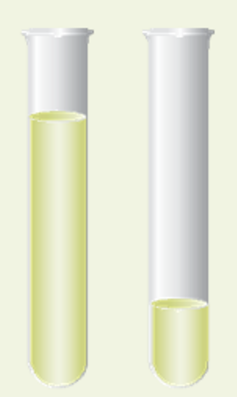
\includegraphics[width=0.25\textwidth]{./images/unusual-liquid.png}
            \caption{Unusual Liquid Watch}
            \label{liquid}
        \end{figure}

        We can start by dividing each tubes into equal parts, and then fill up based on the time shown.
        We can illustrate it as such (figure \ref{liquid_annotated}). The left tube is divided based on each hour and the right tube is divided based on every 15 minutes
        \begin{figure}[h]
            \centering
            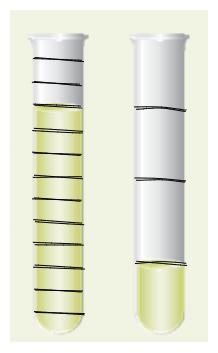
\includegraphics[width=0.25\textwidth]{./images/liquid-annotated.png}
            \caption{Liquid with Marks}
            \label{liquid_annotated}
        \end{figure}

        \pagebreak

        After we divide the tubes into equal parts, we can make draw colour over them (figure \ref{liquid_filled}) that (roughly) represents 4.20

        \begin{figure}[h]
            \centering
            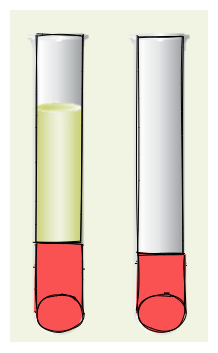
\includegraphics[width=0.25\textwidth]{./images/liquid-filled.png}
            \caption{Liquid with Marks}
            \label{liquid_filled}
        \end{figure}
    }
    \item {
        Students at the school must decide what subjects they will study next year.
        English, science, and Math are all compulsory, but they can choose from the remaining four subjects.
        Table \ref{choice_table} shows how choices can be made. Students must select one subject from each column.
        The fourth subject can come from any column.

        \setcounter{table}{4}
        \begin{table}[h]
            \caption{Choices that can be made}
            \label{choice_table}
            \begin{longtabu} to \textwidth {|c|c|c|}
                \hline \multicolumn{1}{|c|}{\textbf{1}} & \multicolumn{1}{c|}{\textbf{2}} & \multicolumn{1}{c|}{\textbf{3}} \\ \hline 
                \endfirsthead

                Geography & French & History \\
                Technology & German & Religious Study \\
                Art & & Physical Education \\
                Music & & Latin \\

                \hline
            \end{longtabu}
        \end{table}

        Which of the following combinations is not allowed?
        \begin{enumerate}[label=\Alph*.]
            \item French, Geography, Physical Education, Art
            \item French, German, Latin, Music
            \item Technology, German, Art, History
            \item French, German, Geography, Music
            \item Geography, Music, French, Religious Studies
        \end{enumerate}

        First thing first, we can check if the first 3 comes from different column.
        After checking each one, we can see that \textbf{D} has incorrect choice. It doesn't have a subject from the third column
    }
\end{enumerate}

\end{document}

